\chapter{Additional Extensions and Applications}
\label{ch:mischelperapps}

In this chapter we describe several applications developed in our SmILE\footnote{\url{http://smile.deri.ie}} group at DERI, and to which we contributed. They are extensions to the work presented in the preceding pages, providing or serving as test use cases and validation scenarios.

We start with a list of extensions to SemNotes' functionality, which employ Natural Language Processing techniques. They focus on specific use cases of note-taking, like ontology engineering, meeting minutes or status reports; as well as text analytics tailored to short text.

The work presented in Chapter \ref{ch:sdwod} was initially motivated by the increasingly difficult task of managing publications on the desktop and on the Web, and the need of connecting the information available in both worlds. \emph{Sclippy} is a tool created to avail of the rich information available on the Web about publications, and bring it to the user's desktop. 
The algorithm described in Chapter \ref{ch:sdwod} is a generalisation of the algorithms used in Sclippy\footnote{\url{http://smile.deri.ie/projects/sclippy}}, extending the scope from publications to any type of desktop resources.

We continue by presenting Konduit, a desktop-based platform for visual scripting with RDF data. Based on the idea of the Semantic Desktop, non-technical users can create, manipulate and mash-up RDF data with Konduit, and thus generate simple applications or workflows, which are aimed to simplify their everyday work by automating repetitive tasks. The platform allows to combine data from both the Web and the desktop and integrate it with existing desktop functionality.

\section{Natural Language Extensions for SemNotes}
\label{sec:nlpsemnotes}

During its development phases, SemNotes has served as a sandbox environment and testing bench for several technologies and prototypes developed within our group. Three of the most notable extensions are related to Natural Language Processing (NLP) of the notes, to add functionality. These include: 
\begin{itemize}
 \item a text analytics extension for keyphrase extraction \cite{Schutz2008}
 \item two controlled language extensions for semantic annotation of meeting minutes and status reports \cite{Davis2008,Davis2009}
\end{itemize}

\subsection{Keyphrase Extraction}

Tagging is one of the most used basic features offered by Nepomuk-KDE and by SemNotes. Tags are important for categorisation and organisation of resources, especially for personal notes. Tagging requires users to make a decision on what is relevant about the resource being tagged and how they might reuse the annotation in the future --- i.e. is the tag expressive enough to be later user for filtering the information and finding the required resource. To support users in their choice of tags, and partially automate it, we collaborated on a keyphrase extraction extension to SemNotes. It is based on the TextAnalytics service developed by \cite{Schutz2008}. 

Keyphrase extraction is just one of the NLP functionalities provided by the Text\-Analytics desktop service, alongside information extraction and speech act detection. The service can be accessed by all desktop applications and is available also as an Eclipse plugin for the Java implementation of Nepomuk.

Standard information extraction tools usually extract information which is already known --- like detecting resources in the text. This is the norm in SemNotes as well, where only known existing desktop resources are suggested as annotations of notes, even when other resources might be referred to, but are unknown to the system. The TextAnalytics service is different and complementary, by extracting terms and instances from text, which are not already known to the system. The new terms can become new desktop resources, once identified.

\begin{figure}[tb]
 \centering
 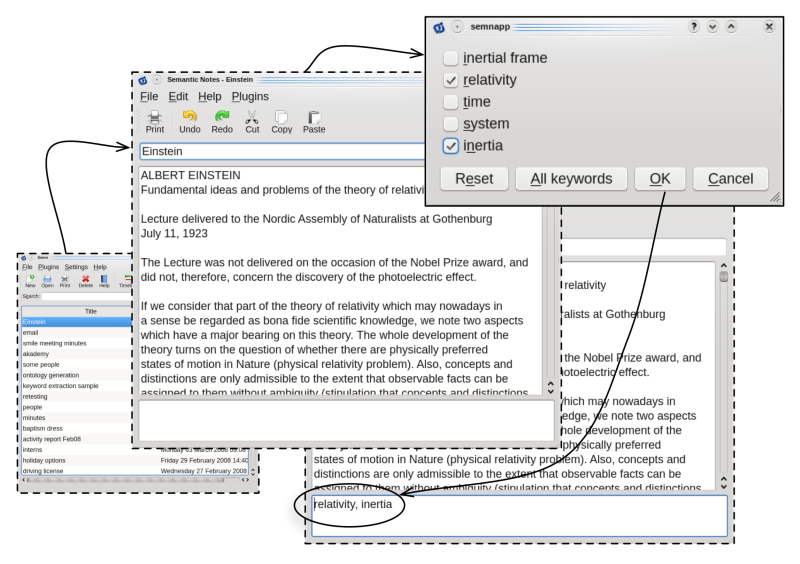
\includegraphics[width=\linewidth]{chapters/core/img/keywordextraction}
 \caption{User interface to keyphrase extraction in SemNotes.}
 \label{fig:keywordextraction}
\end{figure}

We have developed an extension to SemNotes, which uses the service to extract keyphrases from the text of the personal notes and suggest them to the user as tags. The text of personal notes can be small, thus adding difficulty to the extraction task. \cite{Schutz2008} details the way this challenge is tackled in the service. In SemNotes, the service can be called through the menu, and once the note is parsed the relevant terms found are presented to the user as tag suggestions. Figure \ref{fig:keywordextraction}, taken from \cite{Schutz2008}, shows a screenshot of the interface in an older version of SemNotes. If the user accepts any of the suggestions, they become tag resources and are stored in Nepomuk in the usual way.

\subsection{Controlled Language Extensions}

Controlled Natural Languages are well-defined subsets of a natural language with a restricted grammar and lexicon \cite{Schwitter2005}, in order to reduce ambiguity and complexity. In his Ph.D. thesis \cite{Davis2012PhD}, researches the use of Controlled Languages for ontology engineering and semantic annotation. We used SemNotes for prototype testing of both directions, while also providing a feasible use case for the services.

SemNotes, as a note-taking application, is well suited for Controlled Language use, since the main type of input from the users is textual. As a Semantic Desktop application it is also particularly well suited to ontology engineering due to the direct access provided by the framework to the underlying ontologies and desktop resources. As an annotation tool it is also a good testing ground for the semantic annotation using Controlled Language.

\subsubsection{Round Trip Ontology Authoring}

Controlled Natural Language proved efficient for creating ontologies in a user friendly way, for naive users who do not wish or do not need to learn how to use full-fledged ontology editors, nor want to dive into the complexities of ontology engineering. However simplified, Controlled Languages still require that the users be familiar with the vocabulary and syntax rules in order to use the language properly. The Round-trip Ontology Authoring environment described in \cite{Davis2008} aims to reduce the learning curve required to use Controlled Languages for ontology authoring. It combines and builds on the CLOnE controlled language for ontology editing \cite{Funk2007}, and Natural Language Generation from existing ontologies, to provide a simplified process: starting with an existing ontology, either imported or produced using CLOnE, generate the Controlled Language, edit the text, then parse it back into the modified ontology. Since the user only has to work with the textual representation of the ontology, we created a prototype extension for SemNotes to test the process.

Our extension allowed all the steps of the process --- import of existing ontologies, editing and exporting back into an ontology. It also had the added benefit of having access to all the ontologies loaded on the Semantic Desktop, and all the instances extracted from the personal data available on the desktop. Thus SemNotes allowed reuse of existing instances from the desktop in the ontology editing, and more importantly to create instances directly into the desktop repository, in a simple and user friendly way. It also meant that through this extension we could provide a way of easily creating or removing a relation between existing instances just by typing a sentence about it. 

\subsubsection{Controlled Language Annotation}

As we described before, SemNotes provides semi-automatic annotation of notes, by checking the available desktop resources and suggesting instances which are relevant to the note. Semi-automatic annotation is a mechanism often used to simplify the process of semantic annotation, and support the user. By employing Controlled Natural Language techniques, we can improve further the annotation process, in a user-friendly way. \cite{Davis2009} presents two approaches to applying Controlled Language to Semantic Annotation, called CLANN --- Controlled Language ANNotation. The two approaches were used to measure and evaluate the balance needed between expressiveness of the language and ease of use. CLANN is based on CLIE (Controlled Language for Information Extraction) and CLOnE. 

Semantic annotation with Controlled Language is better suited for some annotation scenarios than for others. CLANN is applied to two use cases, where the use of a controlled vocabulary is implicit --- meeting minutes and status reports. However, other possible use cases include the eHealth and business domains. The two use cases benefit from a semantic note-taking tool like SemNotes, thus creating an extension that uses CLANN was the next logical step.

The CLANN extension of SemNotes allows users to simultaneously create and annotate meeting minutes or status reports in Controlled Natural Language. It goes beyond the initial interlinking capabilities of SemNotes, by allowing the creation of different relations between the notes and desktop resources, as well as the creation of new resources and relations. CLANN uses a specially designed ontology for the meeting minutes and status reports, called MEMO, which is based on the desktop ontologies described in Section \ref{sub:nepomuk}. The notes must follow a specific template, which is then parsed by the service. In the parsing, the extension reuses SemNotes' mechanism for detecting related desktop resources. The information resulted from the parsed note is stored in the desktop repository.


\section{Linking Publication Data with Sclippy}

The work presented in Chapter \ref{ch:sdwod} is based on previous work \cite{Groza2009} on linking publication data from the Web of Data and from the Semantic Desktop. It consists of a three step process (extraction, expansion, integration) that starts from a file with no metadata and incrementally enrich it to a comprehensive semantic model around the given publication, linked and embedded within the personal information space. The process is implemented by Sclippy. 

The three steps are: 
\begin{itemize}
 \item extraction --- metadata is automatically extracted from the publication; 
 \item expansion --- the extracted metadata is used to search the Web of Data and find relevant information which is then connected to the original metadata; and 
 \item integration --- the metadata is further enriched by embedding it within the Semantic Desktop, where it is automatically linked with the existing personal metadata.
\end{itemize}

The work done by \cite{Groza2009a} is broader in a sense than our work, as it also includes in the first step of the process --- extraction --- containing complex algorithms for shallow (i.e. title, authors, abstract) and deep (i.e. discourse knowledge items like claims, positions or arguments) extraction of metadata from documents. Our work relies on the metadata already extracted by external applications or by the underlying Semantic Desktop, and instead focuses on the expansion and integration steps. We also aimed to provide a generic model for the integration of Web of Data sources and the Semantic Desktop, broadening the scope from the world of publications and authors.

The linking of publications done by Sclippy was motivated by the growing difficulty for early stage researchers to determine relevant work in a domain. The existing efforts are limited in the online world, where there are many publishers, each providing access to disjunct corpora of publications, and regardless of how well interconnected and easy to search they are, they do not cover all possible sources. The Semantic Desktop, being the implicit place where researchers would store documents, and already providing means of interlinking and better management of information, is the obvious choice for connecting to the similar but richer information available on the Web.

While Sclippy served as basis for our work, it also provided our first real-world use case where the interlinking of the Semantic Desktop data with the Web of Data would be useful, as well as the first example of a customised desktop service benefiting from it.


\section{Building User-Applications with Konduit}

An added benefit of structured information is its potential for reuse: being able to integrate existing data, relieves users from creating it again. While a large part of the data is found online, when it comes to working with information, users still rely on the familiar environment of desktop-based applications. On the other hand, Web-based applications can only access Web data, and do not integrate well with desktop information.

Konduit \cite{Dragan2009b} offers a way of accessing structured Web data from the desktop, integrating it with existing desktop data and applications, and working with both in a unified way. It precedes the system for finding Web aliases for semantic resources from the desktop, presented in Chapter \ref{ch:sdwod}. 

The goal of Konduit was to allow the users to easily design their own personalised applications, customised to their needs and based on their workflows, without requiring prior knowledge of programming languages, or even semantics.
Our approach with Konduit is based on a combination of the visual programming paradigm and the idea of UNIX pipes, and allows the casual users to build simple programs in order to perform and automate everyday tasks on RDF data. In other words, it is visual programming for RDF. 

\subsection{Components and Workflows}
\label{sec:konduit_components_and_workflows}

Konduit provides a collection of useful components ready for immediate use. The components offer individual units of functionality and are represented visually as blocks. They are connected through input and output slots, and in this way the flow of the program is defined. In order to keep simple the task of connecting components, the only data that flows through the workflow is RDF. This condition ensures that each component always fulfils the minimal requirement for dealing with its input. Obviously, components may be specialised with respect to the actual vocabulary on which they can operate and will decide at runtime if and how they deal with the incoming RDF. By neither allowing different kinds of data (e.g., text, numbers, lists, images, etc.), nor typing the RDF data with respect to the vocabularies they use, we stay very close to the original UNIX pipes concept, where data is always an untyped stream of bytes, and where it is up to each process or program how to handle it. 

The architecture of Konduit is modular, each component is realised as a plugin which can be independently installed or removed. We expect that new plugins will be developed and shared by external power users, as the need for them arises. 
Formally, a component is defined by the following parameters:
$$
Component = (I, O, P, F )
$$
\begin{itemize}
 \item a set of RDF input slots $I$,
 \item a set of RDF output slots $O$, 
 \item a set of parameters $P$ which allow for user input in the workflow, 
 \item a function $F$, which works on the input $I$ and generates the output $O$.
\end{itemize}
The parameters $P$ influence the behaviour of $F$.

The number of input and output slots is not fixed and can be 0 or more. Depending on the number of slots, components can be grouped in three categories: sources, sinks, and ordinary components. Sources are components that do not have any inputs. They supply the workflow with data. There is always at least one source at the start of any workflow. Because data graphs can be merged, there can be more than one source for any workflow. Typical examples of sources are connectors to RDF stores, file (URL) input components, or converters from other, non-RDF formats. Sinks are components that do not have any outputs. They represent the final point(s) of any workflow. Examples of sink components are application adaptors, serialisers (file output components) and visualisers. In Konduit, workflows are activated from a sink component, usually by clicking on an activation button.

Several connected components make up a workflow, which is defined by specifying
$$
Workflow = (C, f) , where f: inputs(C) \rightarrow outputs(C) \cup \{~nil~\}
$$
\begin{itemize}
 \item a set of components $C$,
 \item a function $f$ defined from the set of all the inputs of the components of $C$ to the set of all the outputs of the components of $C$ and the $nil$ output.
\end{itemize}
The function $f$ shows how the components of $C$ are connected. The inputs that are not connected have a $nil$ value of $f$; the outputs that do not represent a value of $f$ are not connected.

Workflows can be saved and reused. Saving a workflow implies saving all the components that have at least one connection to it, as well as their existing connections, parameters and layout. There is no restriction that the components should be completely connected, so there can be input or output slots that remain open. A saved workflow can be reopened and modified by adding to it or removing components, or by changing connection or parameters and thus obtaining different workflows with minimum effort.

An important aspect of Konduit is directly tied to the fact that all inputs and outputs are RDF graphs. As a result, any workflow can itself become a component, meaning that workflows can be built recursively. In this way, it is possible to create specialised components, which we call black boxes, based on the combination of other components. The blackboxes are added to the existing library for reuse. An example of saved workflows and blackboxes is shown in Figure \ref{fig:discography_generator}. The workflow is taken from \url{http://smile.deri.ie/konduit/discography}, where an entire example use case is presented.

\begin{figure}[!ht]
 \centering
 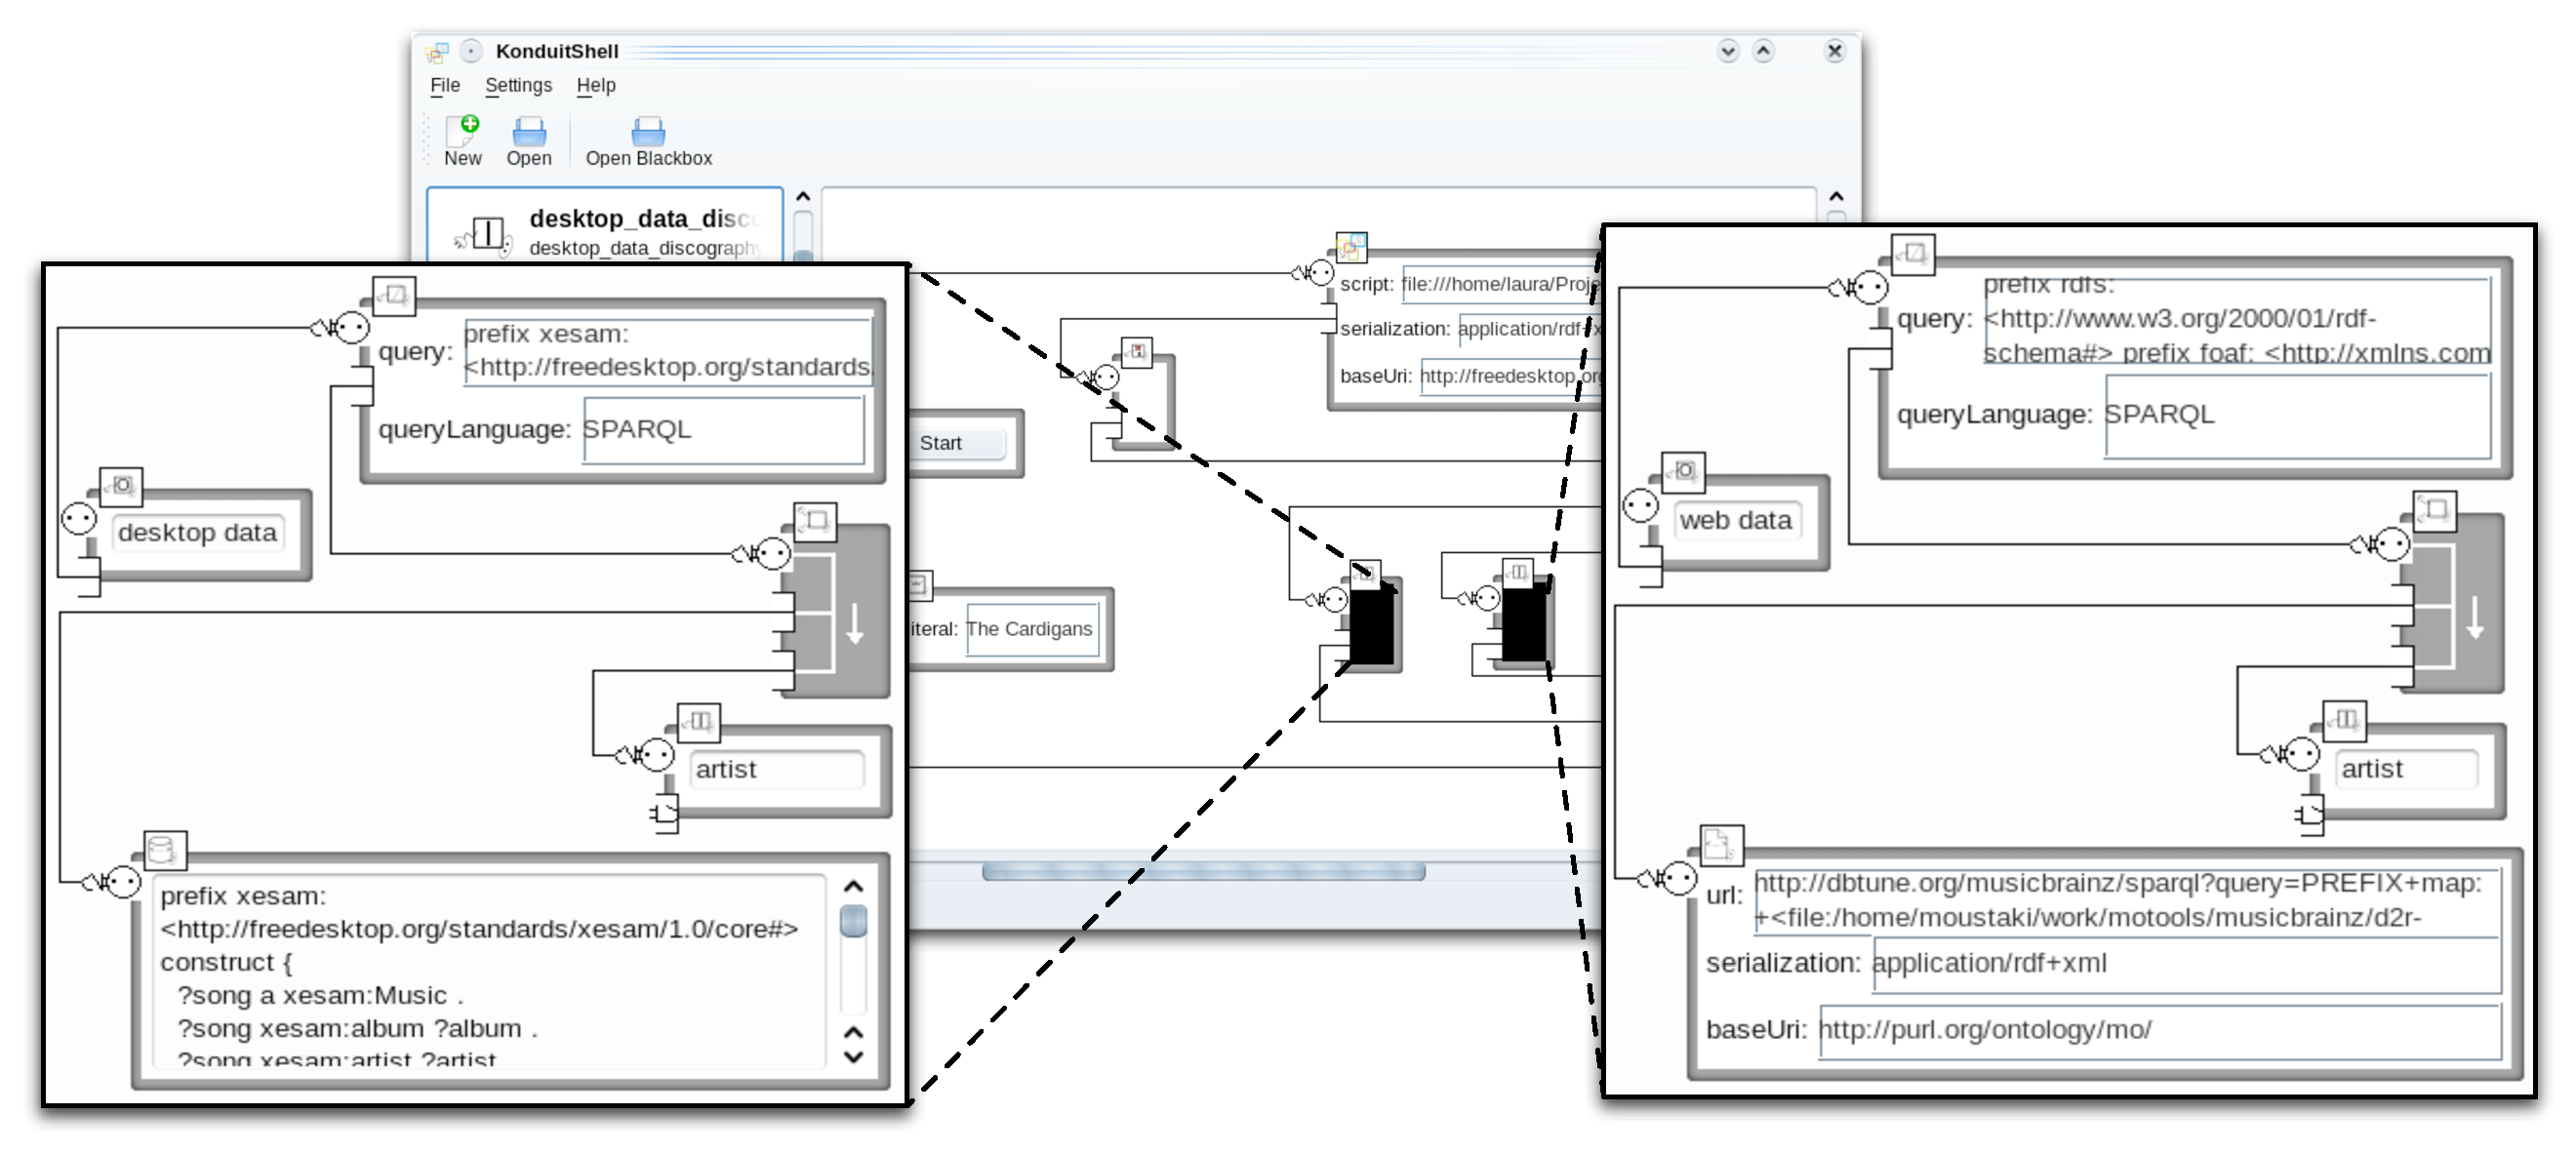
\includegraphics[width=1.0\linewidth]{chapters/core/img/discography}
 \caption{The entire discography generator workflow.}
 \label{fig:discography_generator}
\end{figure}

\cite{Dragan2009b} describes in more detail the different types of sources, sinks, and ordinary component types, as well as the blackbox mechanism. 
Some of the basic components available for Konduit require previous knowledge of writing SPARQL queries. Since the queries can influence the performance of the entire workflow, we recognise the need for a smart query editor that is suitable for naive users. \cite{Ambrus2010} describes the means for making Konduit more user friendly, by adding a smart wizard with suggestions and SPARQL autocompletion. 

